\documentclass{cahier_des_charges}
\usepackage{lipsum}
\usepackage{hyperref}
\usepackage{enumitem}
\usepackage{titlesec}
\titleformat{\section}{\large\bfseries}{\thesection}{1em}{}
\titleformat{\subsection}{\normalsize\bfseries}{\hspace{1em}\thesubsection}{1em}{}
\titleformat{\subsubsection}{\small\bfseries}{\hspace{2em}\thesubsubsection}{1em}{}
\title{Cahier des charges - L2I1} %Titre du fichier

\begin{document}

%----------- Informations du rapport ---------

\titre{Cahier des charges \\ L2I1 - Tamagotchi} %Titre du fichier .pdf
\UE{UE Projet de programmation} %Nom de la UE
\sujet{Projet L2I1 - Tamagotchi} %Nom du sujet

\encadrant{Camille \textsc{KURTZ}} %Nom de l'enseignant
\responsable{David \textsc{JANISZEK}}

\auteurs{Marwan \textsc{DENAGNON} \\
		Lina \textsc{BOUGUETTAYA} \\ 
		Yasmine \textsc{DEHOUCHE} \\
		Abhijeet \textsc{SINGH}} %Nom des élèves

%----------- Initialisation -------------------
        
\fairemarges %Afficher les marges
\fairepagedegarde %Créer la page de garde
\renewcommand{\contentsname}{Sommaire}
\tableofcontents %Créer la table de matières
\newpage


%------------ Corps du rapport ----------------


\section{Introduction} 

Dans le cadre de notre projet de L2 Informatique, nous avons développé une application innovante qui revisite le concept du Tamagotchi, cet animal virtuel interactif qui a marqué les esprits depuis les années 90. Notre ambition est de moderniser ce classique intemporel en intégrant des fonctionnalités inédites, adaptées aux technologies d’aujourd’hui, pour offrir une expérience à la fois plus immersive et plus engageante.

Le Tamagotchi original, lancé dans les années 90, était un petit appareil électronique portable qui permettait aux utilisateurs de nourrir, divertir et prendre soin d’un animal virtuel. Avec l’évolution des technologies mobiles et des smartphones, nous avons l’opportunité de repenser complètement cette interaction. Notre application transforme cette expérience nostalgique en un compagnon virtuel moderne, connecté et accessible à tous.


\section{Guide de lecture}

\subsection{Maîtrise d’œuvre}
\subsubsection{Responsable}
Nom de l'encadrant : Kurtz Camille 

Le maître d’œuvre analyse les propositions du groupe et supervise le développement de l'application web.
l'application web.
\subsubsection{Personnel technique}
Les personnes oeuvrant pour ce projet sont des étudiants en deuxième année de licence informatique :
\begin{itemize}[label=\textbullet]
\item Lina BOUGUETTAYA 
\item Yasmine DEHOUCHE
\item Marwan DENAGNON 
\item Abhijeet SINGH
\end{itemize}
\subsection{Maîtrise d'ouvrage}
Dans le cadre de ce projet la maitrise d’ouvrage est assurée par l’encadrant Camille Kurtz.
\section{Concepts de base}
L’application à concevoir est un jeu mobile Android inspiré des Tamagotchis classiques, des gadgets qui, en appuyant sur des boutons situés autour d'un petit écran vidéo, permet de nourrir, laver et soigner l'animal virtuel pour qu'il « vive » le plus longtemps possible. L’objectif principal de cette application est de moderniser les Tamagotchis originaux, en ajoutant des fonctionnalités qui exploitent les capacités technologiques de nos smartphones. Notre application sera développée à l’aide des techniques suivantes :
\begin{itemize}[label=\textbullet]
\item Java
\item XML
\item JSON
\end{itemize}
Vous pouvez retrouver la définition de ces termes dans la partie \protect\hyperref[sec:glossaire]{Glossaire}

\section{Contexte}
De nos jours, il n’est plus nécessaire d’acheter des jeux physiques. Tout type d’applications existent sur nos téléphones portables. Dans ce cadre, on souhaite développer un jeu emblématique des années 90, le Tamagotchi en version virtuelle. Ce projet vise à développer une application mobile android sur laquelle on peut prendre soin d’un animal fictif et le transmettre à quelqu’un d’autre lorsqu’on ne peut plus prendre soin de lui.
Notre groupe de projet L2I1 est encadré par Mr Camille KURTZ, et composé de 4 étudiants:
\begin{itemize}[label=\textbullet]
\item Lina BOUGUETTAYA


\item Yasmine DEHOUCHE


\item Marwan DENAGNON


\item Abhijeet SINGH
\end{itemize}
\section{Historique}
Le Tamagotchi a été inventé en 1996 par l’entreprise japonaise Bandai, qui est une entreprise de jouets (un autre succès de Bandai est par exemple les jouets Power Rangers). 
Tamagotchi traduit en français signifie « œuf » (tamago) « montre » (wotchi). Comme son nom l’indique il s’agit donc d’une sorte de montre (donc portable) dans laquelle on doit s’occuper d’un œuf afin qu’il éclose pour pouvoir jouer avec lui. 
On peut le nourrir, le caresser, le nettoyer et faire divers mini-jeux en sa compagnie, le « but » principal du jeu est de maintenir son compagnon en bonne santé et de le faire vivre le plus longtemps possible, si l’on échoue, le jeu recommencera avec un nouvel œuf et donc un nouveau compagnon.
\section{Description de la demande}
\subsection{Les objectifs}
Le projet à réaliser consiste à concevoir une application mobile sur Android appelée « Tamagotchi », où l’utilisateur aura pour but de s’occuper d’une créature virtuelle ayant plusieurs caractéristiques.
Le tamagotchi sera caractérisé en premier lieu par une jauge de faim ayant pour états (Ok, affamé, mort). Ensuite, l’utilisateur devra pouvoir réaliser d’autres fonctionnalités sur sa créature telles que : guérir, dormir et laver, qui décriront ses différents états (malade, fatigué, sale).
De plus, des interactions supplémentaires seront mises en place telles qu’une baisse de santé en cas de fatigue.
Enfin, l’utilisateur devra avoir la possibilité de transférer son Tamagotchi à un autre utilisateur et de faire interagir deux Tamagotchis via NFC ou une base de données externe.
\subsection{Produit du projet}
L’application Android créée sera un outil ludique de divertissement, permettant aux utilisateurs d’adopter un animal et d’en prendre soin. Ce projet a pour but d’offrir l’expérience nostalgique avec une touche moderne du jeu TAMAGOTCHI, en ciblant un public jeune et amateur de jeux mobiles. Elle permet aux joueurs d’adopter, nourrir, nettoyer, soigner et interagir avec son compagnon virtuel. Elle contiendra des fonctionnalités telles que la transmission des animaux via NFC. Le produit sera entièrement gratuit, exploitant des technologies open-source et des services sans frais pour donner un accès plus affordable à un public plus important.
\subsection{Les fonctions du produit}
\subsubsection{Fonctionnalités indispensables}
\begin{itemize}[label=\textbullet]
\item Système de gestion
\begin{itemize}[label=\textendash]
\item F0 : Persistance des données et traitement en arrière-plan pour assurer un fonctionnement continu.
\end{itemize}
\item Interaction avec l’animal
\begin{itemize}[label=\textendash]
\item F1 : Création d’un tamagotchi avec un nom et un choix parmi plusieurs options.

\item F2 : Affichage des jauges de faim et de bonheur, initialisées à 100.

\item F3 : Possibilité de nourrir l’animal.

\item F4 : Possibilité de laver l’animal.

\item F5 : Possibilité de guérir l’animal en cas de maladie.

\item F6 : Possibilité d’endormir l’animal.
\end{itemize}
\item Gestion des données
\begin{itemize}[label=\textendash]
\item F7 : Saisie et modification des données du tamagotchi.

\item F8 : Lecture et consultation des données enregistrées.

\item F9 : Sauvegarde des données pour conserver la progression.

\item F10 : L’animal meurt s’il est négligé (jauges critiques).
\end{itemize}
\end{itemize}
\subsubsection{Fonctionnalités optionnelles}
\begin{itemize}[label=\textendash]
\item FO1 : Gestion de l’âge du tamagotchi.

\item FO2 : Importation et exportation d’un animal.

\item FO3 : Attribution de bonus quotidiens à chaque connexion.

\item FO4 : Affichage de bulles d’émotions pour exprimer l’état de l’animal.
\end{itemize}
\subsubsection{Fonctionnalités perspectives}
\begin{itemize}[label=\textendash]
\item FP1 : Possibilité de gronder l’animal en cas de mauvais comportement.

\item FP2 : Intégration de mini-jeux pour interagir avec l’animal.

\item FP3 : Ajout de musique d’ambiance pour enrichir l’expérience utilisateur.
\end{itemize}
\subsection{Critères d’acceptabilité et de réception}
\begin{itemize}[label=\textbullet]
\item L'utilisateur doit pouvoir nourrir, nettoyer et jouer avec son Tamagotchi.
\item Les statistiques (faim, bonheur, santé, propreté) doivent évoluer en temps réel.
\item L'interface doit être simple et facile à comprendre, même pour des enfants.
\item Des tests utilisateurs doivent être réalisés pour valider l'expérience globale.
\end{itemize}
\section{Contraintes}
\subsection{Contraintes de coûts}
Ce projet a été conçu pour être entièrement gratuit, en utilisant des technologies et des services gratuits, afin de garantir qu'aucun coût ne soit engagé.
\subsection{Contraintes de délais}
Le projet s'étalera sur une durée totale de 12 semaines, au cours desquelles différentes phases de planification, d'exécution et d'évaluation seront mises en œuvre afin d'assurer son bon déroulement et l'atteinte des objectifs fixés.
\subsection{Contraintes matérielles}
La réalisation de ce projet inclue l’utilisation d’une interface tactile (Smartphone, tablette) fonctionnant sous Android afin de tester le jeu et d’ordinateurs pour le développement. Une connectivité mobile sera indispensable pour la synchronisation des données notamment pour le transfert et l’interaction entre Tamagotchis via NFC.
De plus, une base de données locale et/ou externe pour assurer la persistance des informations et la gestion des interactions à distance.
\subsection{Autres contraintes}
\subsubsection{Contraintes techniques}
\begin{itemize}[label=\textbullet]
\item L’optimisation de la performance avec une gestion efficace des ressources (mémoire, CPU, GPU), afin d’éviter les ralentissements et les crashs.
\item Minimiser la consommation d'énergie de l’appareil, en réduisant l’utilisation des animations et des capteurs de mouvements.
\item Prévention d’un mode hors ligne pour que le jeu soit accessible à son utilisateur à tout moment, et une synchronisation dès que la connexion est rétablie.
\item Adaptation de l’interface à différents types et tailles d’écrans.
Fournir une sécurité avec un système de chiffrements des données sensibles, tel que lors des interactions via NFC.
\end{itemize}
\subsubsection{Contraintes fonctionnelles}
\begin{itemize}[label=\textbullet]
\item Notifications de rappel pour s’occuper de son animal.
\item Prévoir un système de QR Code en cas d’instabilité avec la communication NFC.
\end{itemize}
\subsubsection{Contraintes légales et éthiques}
\begin{itemize}[label=\textbullet]
\item Respecter les règlements RGPD et Google Play Policy.
\item Ajout d’une politique de confidentialité claire pour expliquer la collection de certaines données et pourquoi.
\item Prendre en compte que l’application attire un jeune public, par conséquent éviter tout contenu inapproprié.
\end{itemize}
\section{Déroulement du projet}
\subsection{Planification}
\begin{table}[h!]
    \centering
    \begin{tabular}{|c|c|c|c|}
        \hline
        \textbf{Semaine} & \textbf{Date} & \textbf{Tâches} & \textbf{Chef de projet} \\ \hline
        N°1 & 27/01/2025 & Définition des objectifs & Yasmine DEHOUCHE \\ \hline
        N°2 & 03/02/2025 & Analyse des besoins & Abhijeet SINGH \\ \hline
        N°3 & 10/02/2025 & Rendu du cahier des charges & Marwan DENAGNON \\ \hline
        \multicolumn{4}{|c|}{\textbf{Vacances}} \\ \hline
        N°4 & 17/02/2025 & Rendu du cahier de recettes & Lina BOUGUETTAYA \\ \hline
        N°5 & 24/02/2025 & Rendu de la conception détaillée & Yasmine DEHOUCHE \\ \hline
        N°6 & 03/03/2025 & Développement & Abhijeet SINGH \\ \hline
        N°7 & 10/03/2025 & Développement & Marwan DENAGNON \\ \hline
        N°8 & 17/03/2025 & Développement & Lina BOUGUETTAYA \\ \hline
        N°9 & 24/03/2025 & Développement & Yasmine DEHOUCHE \\ \hline
        N°10 & 31/03/2025 & Intégration & Abhijeet SINGH \\ \hline
        N°11 & 07/04/2025 & Rendu du projet & Marwan DENAGNON \\ \hline
        \multicolumn{4}{|c|}{\textbf{Soutenances}} \\ \hline
    \end{tabular}
    \caption{Planification du projet}
    \label{tab:planification}
\end{table}

\subsection{Ressources}
\subsubsection{Ressources matérielles}
\begin{itemize}[label=\textbullet]
 \item Ordinateurs fonctionnels, 
 
 \item Logiciels de développement (IDE)

 \item Un gestionnaire de version (Subversion) 

 \item Connexion internet stable
\end{itemize}
\subsubsection{Ressources humaines}
Les étudiants composant le groupe L2I1

\section{Étude de marché}
\subsection{Publique cible}
\begin{itemize}[label=\textbullet]
\item Enfants (6-18ans) :
Attirés par des expériences interactives et ludiques. Ce public recherche des jeux colorés et
intuitifs avec des interactions amusantes.
\item Adultes nostalgiques (25-40 ans) :
Ayant grandi avec le Tamagotchi des années 90, ils sont sensibles à la nostalgie et aux références
rétro. Ce public est attiré par des jeux simples qui rappellent leur enfance. Ils apprécient
également les jeux sans microtransactions intrusives.
\end{itemize}
\subsection{Fonctionnalités uniques}
\begin{itemize}[label=\textbullet]
\item Transfert temporaire de l’animal :
Une fonctionnalité innovante permettant aux utilisateurs de prêter ou échanger temporairement
leur animal virtuel avec des amis ou des membres de la famille. Cela favorise les interactions
sociales et la création de liens autour du jeu.
\item Microtransactions :
Contrairement à la majorité des jeux mobiles, ce jeu ne propose aucune microtransaction. Cela
garantit une expérience de jeu équitable, sans interruptions ni incitations à dépenser de l’argent.
Ce modèle peut attirer les parents soucieux des dépenses in-app de leurs enfants et plaire aux
joueurs adultes fatigués des achats intégrés.
\end{itemize}
\subsection{Concurrences}
\begin{itemize}[label=\textbullet]
\item Tamagotchi Forever :
\begin{itemize}[label=\textendash]
\item Points forts : Jeu officiel avec la reconnaissance de la marque Tamagotchi,
graphismes professionnels, univers fidèle à l’original.
\item Limites : Présence de microtransactions, ce qui peut rebuter certains utilisateurs.
\end{itemize}
\item My Talking Tom :
\begin{itemize}[label=\textendash]
\item Points forts : Franchise très populaire, graphismes attrayants, nombreuses
fonctionnalités interactives.
\item Limites : Fortement basé sur des achats in-app, ce qui peut frustrer les joueurs
cherchant une expérience gratuite complète.
\end{itemize}
\end{itemize}
\subsection{Positionnement}
Notre jeu se positionne comme une alternative sans microtransactions, favorisant l’interaction
sociale grâce au transfert temporaire d’animaux. Il combine la nostalgie des années 90 avec des
fonctionnalités modernes pour capter un public large, des enfants aux adultes.
\section{Annexes}
\subsection{Github}
Lien Github du projet : \href{https://github.com/Mvrwvn/Tamagotchi-L2I1}{https://github.com/Mvrwvn/Tamagotchi-L2I1}
\subsection{Maquette}
Vous trouverez ci-dessous les pages de l'application, vous trouverez plus de détail sur les images sur le lien dans la section Références.
\newpage
\noindent
\begin{minipage}[t]{0.48\textwidth}
    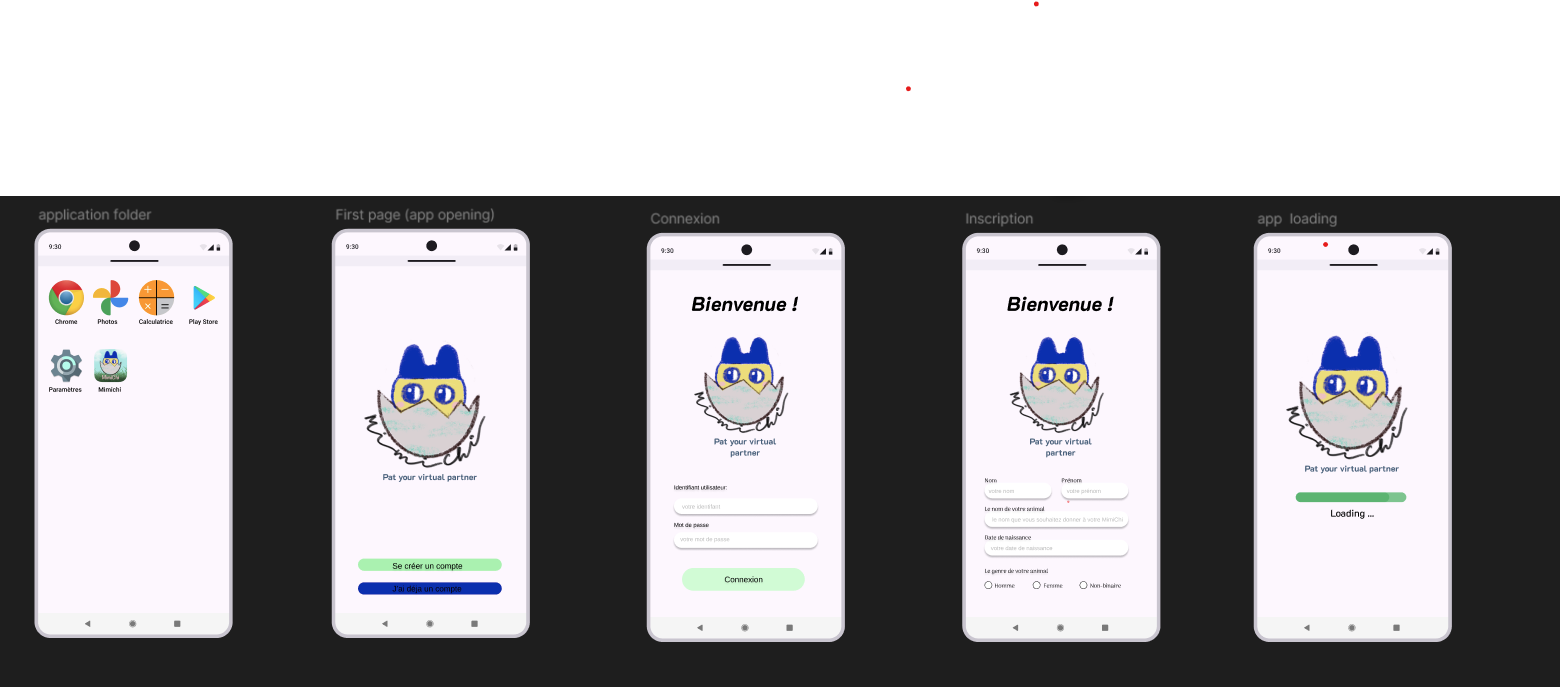
\includegraphics[width=\linewidth]{maquette/screen1.png}
\end{minipage}
\hfill
\begin{minipage}[t]{0.48\textwidth}
    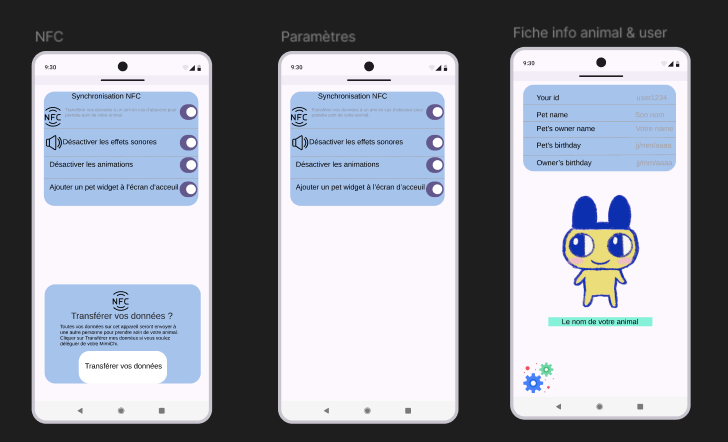
\includegraphics[width=\linewidth]{maquette/screen8.png}
\end{minipage}\par\vspace{0.3cm}

\begin{minipage}[t]{0.48\textwidth}
    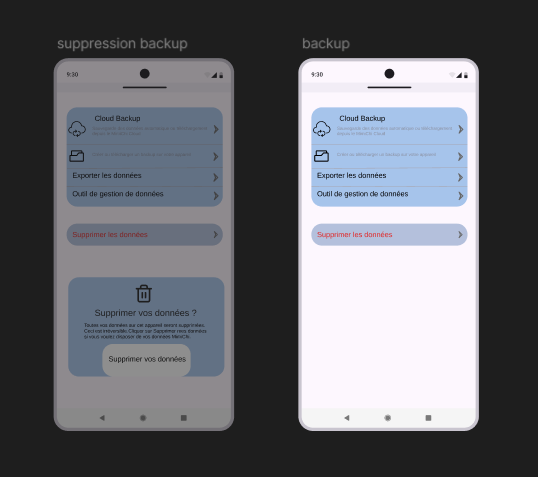
\includegraphics[width=\linewidth]{maquette/screen9.png}
\end{minipage}
\hfill
\begin{minipage}[t]{0.48\textwidth}
    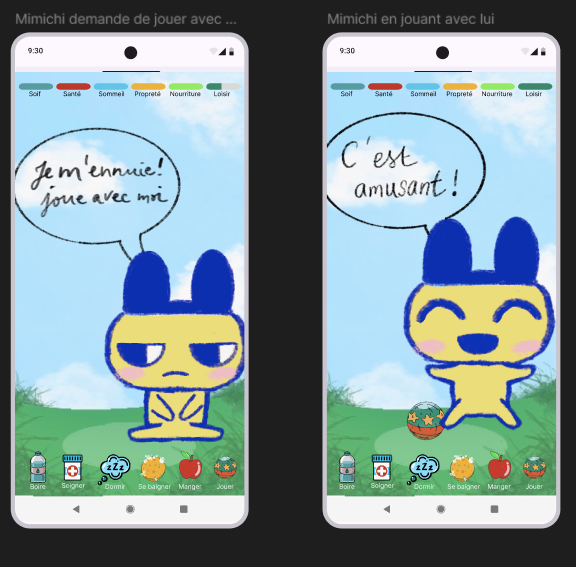
\includegraphics[width=\linewidth]{maquette/screen4.png}
\end{minipage}\par\vspace{0.3cm}

\begin{minipage}[t]{0.48\textwidth}
    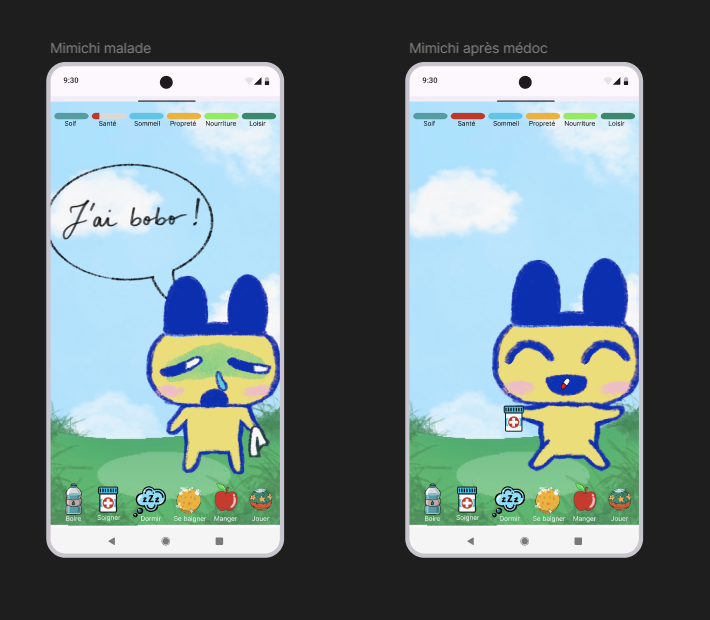
\includegraphics[width=\linewidth]{maquette/screen5.png}
\end{minipage}
\hfill
\begin{minipage}[t]{0.48\textwidth}
    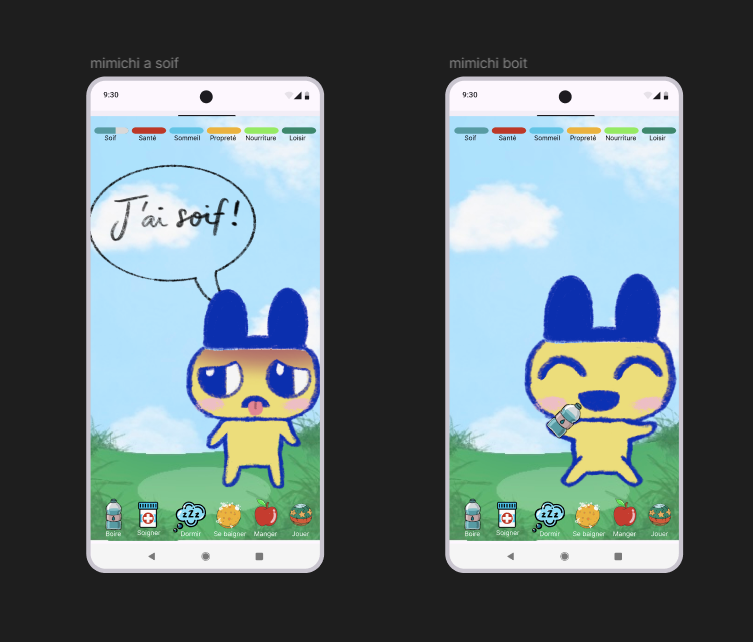
\includegraphics[width=\linewidth]{maquette/screen6.png}
\end{minipage}\par\vspace{0.3cm}

\begin{minipage}[t]{0.48\textwidth}
    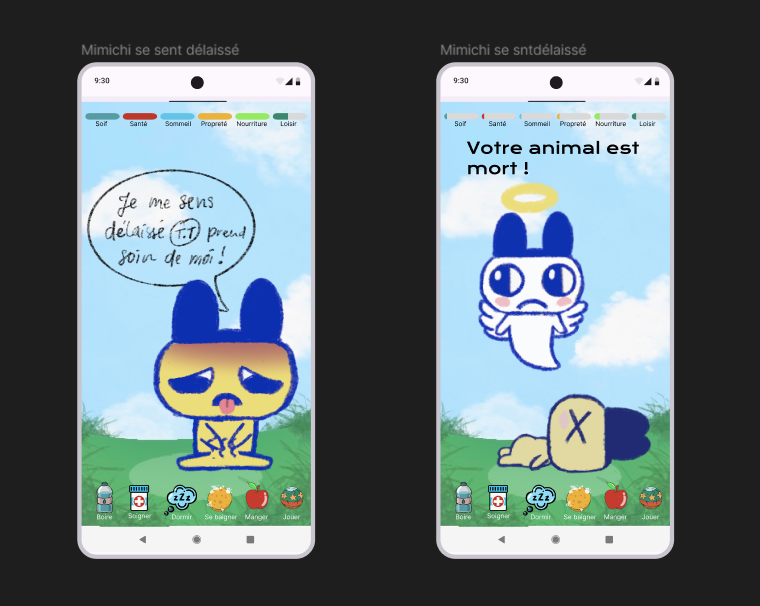
\includegraphics[width=\linewidth]{maquette/screen7.png}
\end{minipage}
\hfill
\begin{minipage}[t]{0.48\textwidth}
    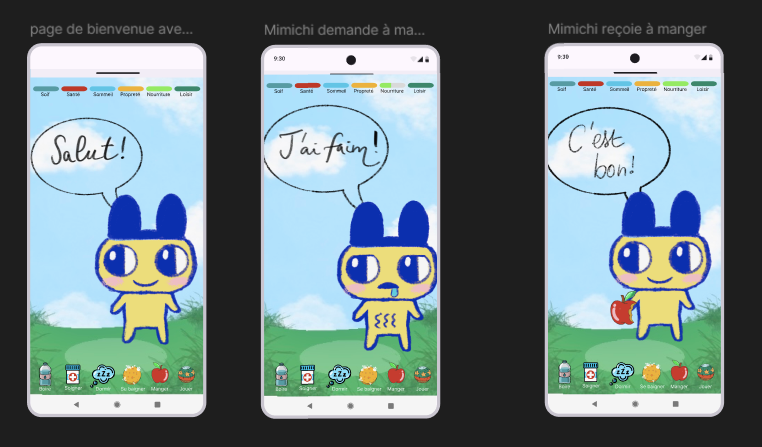
\includegraphics[width=\linewidth]{maquette/screen2.png}
\end{minipage}\par\vspace{0.3cm}

\begin{minipage}[t]{0.48\textwidth}
    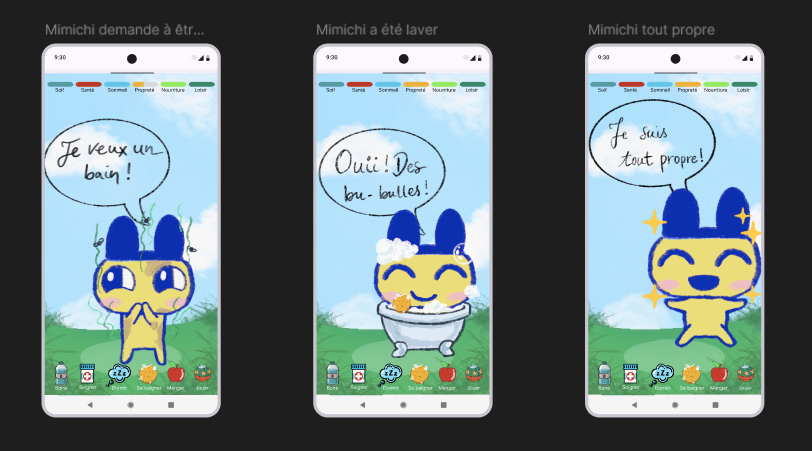
\includegraphics[width=\linewidth]{maquette/screen3.png}
\end{minipage}
\section{Glossaire} \label{sec:glossaire}
\begin{itemize}[label=\textbullet]
\item Application mobile Android : application qui est disponible et manipulable sur un smartphone Android, l’applications et toutes les données nécessaires à son fonctionnement sont stockés en local.
\item Java : Java est un langage de programmation orienté objet, robuste et utilisé pour le développement d'applications Android.
\item XML : Extensible Markup Language est un langage de balisage utilisé pour structurer, stocker et échanger des données dans les interfaces Android et les configurations.
\item JSON : JavaScript Object Notation est un format léger de structuration des données utilisé pour stocker et structurer des données dans une application sans nécessiter de communication avec un serveur. Il peut servir à enregistrer des préférences utilisateur, des configurations ou des bases de données locales.
\end{itemize}

\section{Références} \label{sec:ref}
\begin{itemize}[label=\textbullet]
\item Tamagotchi Wiki \href{https://tamagotchi.fandom.com/wiki/Main_Page}{$https://tamagotchi.fandom.com/wiki/Main_Page$}
\item Android Studio \href{https://developer.android.com/?hl=fr}{$https://developer.android.com/?hl=fr$}
\item JSON \href{https://www.json.org/json-en.html}{$https://www.json.org/json-en.html$}
\item XML \href{https://fr.wikipedia.org/wiki/Extensible_Markup_Language}{$https://fr.wikipedia.org/wiki/Extensible_Markup_Language$}
\item Java \href{https://www.java.com/fr/}{$https://www.java.com/fr/$}
\item Maquette \href{https://www.figma.com/design/koCZsOk1kDRrowfl691SRs/MimiChi-L2I1-projet?node-id=109-1021&t=waYgwSG2iLA7EKha-0}{$https://www.figma.com/design/koCZsOk1kDRrowfl691SRs/MimiChi-L2I1-projet?node-id=109-1021&t=waYgwSG2iLA7EKha-0$} 
\end{itemize}
\end{document}